\documentclass[a4paper]{article}
\usepackage{amsfonts}
\usepackage{amssymb}
\usepackage{graphicx}
\usepackage{epstopdf}
\usepackage{amsmath}
\usepackage[round]{natbib}
\usepackage[numbered,framed]{matlab-prettifier}
\usepackage{filecontents}
\usepackage{bigfoot}
\usepackage[T1]{fontenc}
\usepackage[top=1in, bottom=1.25in, left=1.25in, right=1.25in]{geometry}
\graphicspath{{C:/Users/Yidan/Desktop/MSc/num_sim_assignments}}


\title{Assignment 2\\Numerical Simulation}
\author{Yidan Sun}
\date{\today}          
\begin{document}
	\maketitle
	\section*{part 1}
	\begin{figure}
		\centering
		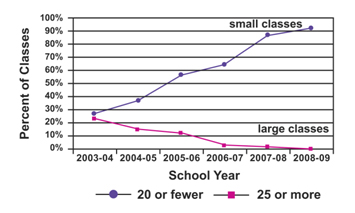
\includegraphics[scale=1]{figure1}
	\end{figure}
	\subsection*{1}
	The authors address several research questions, also because they are discussing two separate experiments. I have identified the following questions, listed from most general to most specific:
	\begin{enumerate}
		\item Can providing inputs that address specific unmet needs in schools improve schooling quality?
		\item What are the effects of a remedial education program, in which a 'balsakhi' works on basic skills with the children, on schooling quality?
		\item What are the effects of a computer-assisted learning program, where children in grade four are offered two hours of shared computer time per week, on schooling quality? 
		\item How cost-effective are both of the programs?
	\end{enumerate}
	
	The authors conduct two experiments that provide additional 'inputs' that specifically target the weaker students. Clearly, it is important to know how cost-effective these programs are, especially considering how much cheaper they are as compared to hiring additional regular teachers. Since the hypothesis is that targeting weaker students might be beneficial, it seems natural to test whether weaker students indeed gain more. 
	 
	\subsection*{2}
	
	Now, for each individual student (analysis at the level of te school is also possible) there are two potential outcomes:
	\begin{itemize}
	\item $y_i^1$ is the outcome when treated
	\item $y_i^0$ is the outcome when non treated
\end{itemize}
Where $y_i$ is a measure of learning outcomes, i.e. test score or improvement in test score over the year. Note the counterfactual nature of potential outcomes. Ideally, we would want to compare the learning outcome of a student if he received the treatment with his learning outcome had he not received the treatment. However, since we cannot turn back time this is impossible. 

More practically speaking, they use what they call a value added specification:
\begin{align}
y_{igjPOST}-y_{igjPRE}=\lambda +\delta D_{jg}+\theta y_{igjPRE}+\epsilon{igjPOST} 
\end{align}
That is, change in the testscore of child $i$ in grade $g$ and school $j$ is regressed on treatment assignment $D_{jg}$ and the respective pretest score. This specification asks whether children that received the treatment increased their testscore more, relative to their pretest score, than children that did not receive the treatment.  

Secondly, they use a difference-in-differences specification(\textbf{only reported in working paper version}):
\begin{align}
y_{igjk}=\lambda +\delta D_{jg}+\theta POST_{k}+\gamma(D_{ig}*POST_k)+\epsilon{igjk} 
\end{align}

Where $k$ indexes the individual tests (pre and post potential treatment). Here the interaction term with parameter $\gamma$ is the treatment effect; it is how much more test scores increased for individuals that received the treatment compared to individuals that did not receive the treatment.  

\subsection*{4}

Estimating equations (1) and (2) generates estimates of the average impact of the program on
all children whose school-grade received a balsakhi. However, there might also be an indirect effect on children that did not get help from the balsakhi, as they will share the classroom with fewer students. This indirect channel could potentially work in two ways: 
\begin{itemize}
	\item A class size effect
	\item A peer quality effect 
\end{itemize}

Since teachers were not prepared to assign the children to potential assignment a priori, without knowing whether or not they were going to get a balsakhi, there might be some selection effect issues. To address this the authors do the following:

The authors start by predicting assignment probability in the treatment schools as a flexible function of the pretest score.
\begin{align}
P_{ijg}=(\pi_0 +\pi_1 y_{ijgPRE}+\pi_2 y_{ijgPRE}^2 +\pi_3 y_{ijgPRE}^3+\pi_4 y_{ijgPRE}^4)*D_{jg}+\omega_{ijg}
\end{align}
Let $M_{ij}$ be the vector $[1,y_{ijgPRE},y_{ijgPRE}^2,y_{ijgPRE}^3,y_{ijgPRE}^4]$.
Where $P_{ijg}$ is a dummy indicating whether a child worked with the balsakhi. 

Consider the following structural equation:
\begin{align}
y_{ijgPOST}-y_{ijgPRE}=\gamma D_{jg} +\tau P_{ijg} +M_{ij} \alpha +\epsilon_{ijg}
\end{align}

Here $\gamma$ is the indirect effect, while $\tau$ is the direct effect of having attended the remedial classes on top of being in a school that was assigned to the treatment group. 

The authors use the predicted assignment probability as an instrument for actual assignment probability and then run an IV regression to estimate the parameters of equation (4). 

The authors conclude that the effect of the program is concentrated on children that were indeed assigned to the balsakhi; they cannot reject the hypothesis that being in a balsakhi school had no effect for children who were themselves not sent to a balsakhi. 

	\section*{part 2}
	\subsection*{a}
	The unconfoundedness assumption is also called the \textit{conditional independence assumption}. Basically, it means that selection into treatment (treatment assignment) is based on observable variables only. Formally:
	\begin{align}
	y_i^0,y_i^1\bot d_i |X_i
	\end{align}
	That is, potential outcomes should be independent of the treatment status, conditional on on observed covariates $X_i$. Put differently, it means that the ones that get assigned treatment are a random sample of the population conditional on $X$. 
	 This implies the following:
	\begin{align}
	E(y_i^0|d_i=1,X_i)=E(y_i^0|d_i=0,X_i)=E(y_i^0|X_i)\\
	E(y_i^1|d_i=1,X_i)=E(y_i^1|d_i=0,X_i)=E(y_i^1|X_i)
\end{align}

To use a real world example, consider the STAR experiment discussed in class. There, students were randomly assigned to different class sizes, however the randomization was done within each school. Hence, treatment assignment was random conditional in each subset of the total population, i.e. within each school, but not necessarily across schools. 
\subsection*{b}
\begin{align}
y_i^0=&\beta+X_i'\gamma+u_i\\
E(u_i)=&E(y_i^0)-\beta-E(X_i'\gamma)\\
\nonumber \\
E(u_i|d_i,X_i)=&E(y_i^0|d_i,X_i)-\beta-X_i'\gamma\\
=&E(y_i^0|X_i)-\beta-Xi_i'\gamma\\
=&\beta+X_i'\gamma+E(u_i|X_i)-\beta-X_i'\gamma\\
=&E(u_i|x_i)=E(u_i)
\end{align}

Where (10) uses the fact that the expectation of $X_i'$ conditional on $X_i,d_i$ is simply $X_i'$, (11) uses the fact that $y_i^0,y_i^1\bot d_i |X_i$, (12) uses equation (8) again and (13) uses the fact that $=u_i\bot X_i$. 
\subsection*{c}
\begin{align}
\alpha_i=&y_i^1-y_i^0\\
E(\alpha_i|d_i,X_i)=&E(y_i^1-y_i^0|d_i,X_i)\\
=&E(y_i^1-y_i^0|X_i)\\
E(\alpha_i|di,X_i)=&E(\alpha_i|X_i)
\end{align}

Here (14) simply uses the definition of $\alpha_i$, (16) uses the unconfoundedness assumption and (17) combines (15) and (16), yielding the result. Hence, if the unconfoundedness assumption holds, no matter if the treatment effect is random or constant, it is uncorrelated to treatment assignment, conditional on the observed covariates $X_i$. 

$\alpha_i$ might for example be the effect of a certain medicine. Perhaps we expect that this medicine might have different effects depending on age. Hence, we could construct several age groups, and then within each age group randomly assign treatment and placebos. $\alpha_i$ might be random because different people might react differently to a medicine, although on average it might have a certain effect. In such a setting, treatment assignment is random conditional on the age group one is in. One could then for example estimate the ATE by running a linear regression. 

		\end{document}